\documentclass[11pt,letterpaper]{article}
\usepackage[margin=0.85in]{geometry}
\usepackage[T1]{fontenc}
\usepackage{amsmath,amssymb,booktabs,graphicx,caption,xcolor}
\usepackage{hyperref}
\hypersetup{colorlinks=true,linkcolor=teal,citecolor=teal,urlcolor=teal,
  pdftitle={Outlier Sensitivity of Envelope TSCP: Controlled rf2 and Crime Experiments}}
\graphicspath{{figures/}}
\captionsetup{font=small,labelfont=bf}
\setlength{\parindent}{0pt}
\setlength{\parskip}{0.28em}
\setlength{\textfloatsep}{14pt plus 2pt minus 2pt}
\setlength{\intextsep}{12pt plus 2pt minus 2pt}
\setlength{\tabcolsep}{5pt}
\renewcommand{\arraystretch}{1.12}
\emergencystretch=2em
\renewcommand{\topfraction}{0.92}
\renewcommand{\bottomfraction}{0.85}
\renewcommand{\textfraction}{0.08}
\renewcommand{\floatpagefraction}{0.80}
\setcounter{totalnumber}{4}
\clubpenalty=10000
\widowpenalty=10000
\newcommand{\Env}{\mathrm{Env}}
\newcommand{\CHR}{\mathrm{CHR}}
\newcommand{\Q}{Q_{1-\alpha}}
\title{Outlier Sensitivity of Envelope TSCP\\[3pt]
\large Controlled rf2 and Crime experiments with training-target standardization}
\author{Experimental analysis report}
\date{September 9, 2026}
\begin{document}
\begin{center}
{\LARGE\bfseries Outlier Sensitivity of Envelope TSCP\par}
\vspace{0.4em}
{\large Controlled rf2 and Crime experiments\par}
{\large with training-target standardization\par}
\vspace{0.6em}
September 9, 2026
\end{center}
\begin{abstract}
We investigate whether a single extreme observation explains the loss of
envelope TSCP to Point CHR in existing multi-output regression experiments.
In rf2, 200 matched random splits with training-target standardization show
that deleting the isolated NASI2 value 78.9 reduces envelope's mean full
prediction volume by 85.55\%, with essentially unchanged joint coverage.
The envelope/CHR ratio of mean volumes decreases from 6.347 to 1.477;
the ranking does not reverse. A screen of eight existing cohorts identifies
Crime as a second candidate. Removing its largest-population community changes
the standardized ratio from 38.615 to 0.101. This numerical reversal is driven
by rare extreme-volume calibration splits: after deletion, envelope is smaller
in 100 of 200 splits, and a descriptive bootstrap interval for the mean-volume
ratio includes one. The evidence supports sensitivity to influential observations,
while distinguishing a reversal in the empirical mean from a consistent advantage
across splits. Neither deletion establishes that the removed record is erroneous.
\end{abstract}

\section{Experimental design and estimands}
The primary questions are whether rf2's isolated extreme observation remains
influential after improving the location model's target weighting, and whether
another existing real-data benchmark exhibits a loss-to-win reversal against
Point CHR. Throughout, ``TSCP'' means the current surface-envelope construction
\cite{methodnote}; the historical separated shortcut is not the proposed method
in these comparisons.

\subsection{Matched deletion and training protocol}
Each condition uses the same 200 original train/calibration/test assignments.
In the deletion condition, only the specified observation is removed from its
assigned partition. All other memberships are preserved; the entire remaining
dataset is not repartitioned. Training transformations and the predictor are
refitted as required. Each pair of methods shares the same fitted predictor
and residual arrays. Original rf2 partitions contain 5,759 training, 384
calibration, and 1,536 test observations; Crime partitions contain 1,426, 95,
and 381, respectively. Deletion reduces exactly one partition by one row.

Both datasets use a jointly fitted multi-output random forest with 200 trees,
maximum depth 16, minimum split size 5, minimum leaf size 2, square-root feature
subsampling, squared-error criterion, bootstrap sampling, and model seed 42.
For standardized training, each target is centered and divided by its population
standard deviation computed on the training partition alone. Predictions are
transformed back to the original target units before residual calibration.
This changes target weighting during fitting; it is not a post-fit rescaling of
prediction regions. The retained rf2 condition required 200 new standardized
fits; the removed condition reuses 200 previously completed standardized fits.
Crime uses original and standardized training in both deletion conditions:
600 new fits and 200 reused original fits.

\newpage
\subsection{Regions, coverage, and volume}
Let $\widehat f$ be the location predictor, $d$ the number of outputs, and
$e_{ij}=|y_{ij}-\widehat f_j(x_i)|$ an absolute residual. Both methods return
nonnegative coordinate thresholds $u_{bj}^{M}$ for split $b$ and method $M$.
Their outcome-space regions and full volumes are
\begin{equation}
 C_b^M(x)=\prod_{j=1}^{d}
 [\widehat f_j(x)-u_{bj}^M,\widehat f_j(x)+u_{bj}^M],
 \qquad V_b^M=\prod_{j=1}^{d}2u_{bj}^M.
 \label{eq:volume}
\end{equation}
All experiments target $1-\alpha=0.90$ joint coverage: an observation is covered
only if all coordinates are covered. Reported coverage is the arithmetic mean
of the 200 split-level coverage estimates. Regions have constant volume within
a split, although their centers depend on the test input. Volumes are products
of \emph{full interval lengths}; they are not the historical half-width products.
Absolute volumes must not be compared across datasets with different units or
output dimensions.

The primary relative-volume statistic is
\begin{equation}
 R=\frac{\overline V^{\Env}}{\overline V^{\CHR}},
 \qquad \overline V^M=\frac{1}{200}\sum_{b=1}^{200}V_b^M.
 \label{eq:ratio}
\end{equation}
A value below one favors envelope in mean volume. We also report the median
of the 200 paired ratios $V_b^{\Env}/V_b^{\CHR}$ and the fraction of splits
with a smaller envelope. These are different estimands and can lead to
different assessments when volumes are highly skewed. Coverage changes are
additionally evaluated on the identical test observations common to each pair,
excluding the removed observation from both denominators.

\section{rf2: strong sensitivity without a ranking reversal}
The retained complete-case rf2 cohort has 7,679 observations and eight outputs.
The removed observation has NASI2 target 78.9, at retained position 3660 and
original dataframe index 4782 (zero-based indexing). The next largest value is
5.62; the median is 3.30 and the median absolute deviation (MAD) is 0.07.
Its modified z-score, $0.67449(y-\operatorname{median}(y))/\operatorname{MAD}(y)$,
is approximately 728.45. Neighboring original rows have values
3.56, 3.53, 3.53, 78.9, 3.54, 3.51, and 3.51. The original ARFF contains the
value, so it was not introduced by the experiment cache. These observations
establish statistical extremeness, without proving a measurement or entry error.

\begin{table}[htbp]
\centering\small
\caption{rf2 with training-target standardization in both conditions.
Coverage is in percent; coverage SD is across splits, in percentage points.
Each row summarizes 200 splits.}
\label{tab:rf2}
\begin{tabular}{llrrrr}
\toprule
Observation & Method & Coverage & Cov.\ SD & Mean volume & Median volume\\
\midrule
Retained & Envelope & 90.052 & 1.715 & 101,671.0 & 24,189.5 \\
Retained & Point CHR & 90.091 & 2.366 & 16,019.1 & 8,790.5 \\
\addlinespace
Removed & Envelope & 90.068 & 1.679 & 14,691.5 & 10,197.1 \\
Removed & Point CHR & 90.017 & 2.402 & 9,944.2 & 5,654.3 \\
\bottomrule
\end{tabular}
\end{table}

Table~\ref{tab:rf2} shows an 85.55\% reduction in envelope mean volume, compared
with 37.92\% for Point CHR. The median within-split envelope reduction is
46.44\%, which is smaller because the mean is more affected by extreme-volume
splits. The mean-volume ratio falls from 6.347 to 1.477. Envelope is smaller
in 45/200 retained splits and 52/200 removed splits. Thus, the outlier explains
substantial inefficiency but does not fully explain the remaining disadvantage.
On common test observations, envelope coverage changes by only $+0.0059$
percentage points, with a descriptive 95\% Monte Carlo interval
$[-0.1305,+0.1422]$ percentage points.

\begin{figure}[htbp]
\centering
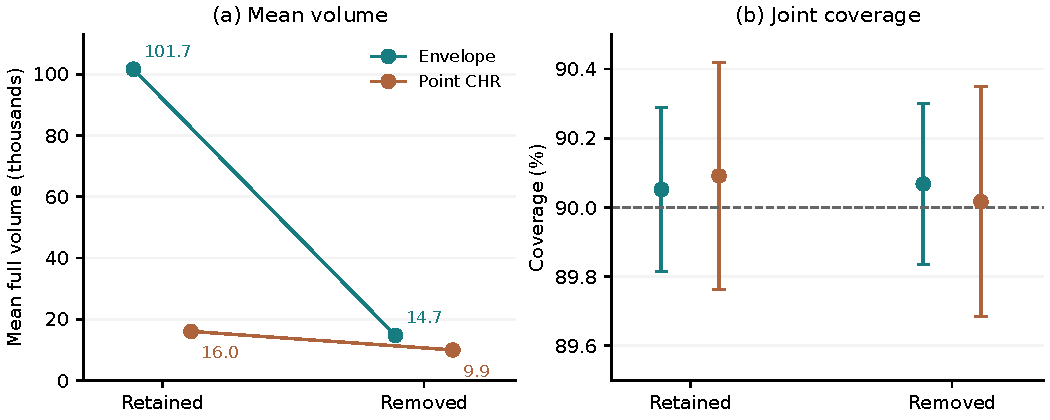
\includegraphics[width=\linewidth]{rf2_control.pdf}
\caption{rf2 under standardized training. Panel (a) shows arithmetic mean full
volume; panel (b) shows mean joint coverage with $1.96\,\mathrm{SD}/\sqrt{200}$
Monte Carlo bars and the 90\% target. The bars describe split variability
conditional on the dataset, not uncertainty for an independently sampled population.}
\label{fig:rf2}
\end{figure}

Training standardization changes the forest's loss weighting but does not
remove the effect of an extreme residual on calibration means and standard
deviations. In the six splits placing the observation in calibration, envelope
mean volume falls from 1,143,702 to 8,622 after deletion. In all 36 test-only
deletions, the training and calibration data are unchanged and the bounds
reproduce identically. Section~\ref{sec:mechanism} separates these roles.

rf2 consists of temporally dependent river-flow observations \cite{mulan}.
The controlled random-split comparison remains informative about sensitivity
under that protocol. It does not establish coverage for a future forecasting
task, where temporal separation and distribution shift require separate
evaluation. A clear outlier-sensitivity effect and a failure to reverse the
method ranking can therefore coexist.

\section{Crime: a qualified reversal in mean volume}
Crime contains community-level records rather than an hourly forecasting
sequence \cite{crime}. The current cohort has 1,902 rows and 18 outcomes,
combining eight crime counts and ten population-based rates. The removal rule
was fixed before examining deletion outcomes: remove the community with the
maximum input population. This is retained position 16, original dataframe
index 21, with population 7,322,564 versus 3,485,398 for the next largest
community. No iterative deletion or threshold search was used to obtain a win.

\begin{table}[htbp]
\centering\small
\caption{Crime under original and standardized target training. All entries
use 200 matched splits and the corrected Point CHR recalibration rank.
Coverage is in percent; volumes use all 18 full interval lengths.}
\label{tab:crime}
\begin{tabular}{lllrrr}
\toprule
Training targets & Community & Method & Coverage & Mean volume & Median volume\\
\midrule
Original & Retained & Envelope & 90.765 & $1.521\times 10^{66}$ & $1.379\times 10^{57}$ \\
Original & Retained & Point CHR & 91.706 & $7.304\times 10^{62}$ & $1.247\times 10^{57}$ \\
Original & Removed & Envelope & 90.803 & $5.406\times 10^{62}$ & $8.106\times 10^{56}$ \\
Original & Removed & Point CHR & 91.665 & $1.529\times 10^{64}$ & $5.178\times 10^{56}$ \\
\addlinespace
Standardized & Retained & Envelope & 90.655 & $7.073\times 10^{65}$ & $1.086\times 10^{57}$ \\
Standardized & Retained & Point CHR & 91.470 & $1.832\times 10^{64}$ & $8.265\times 10^{56}$ \\
Standardized & Removed & Envelope & 90.647 & $5.867\times 10^{62}$ & $4.795\times 10^{56}$ \\
Standardized & Removed & Point CHR & 91.562 & $5.800\times 10^{63}$ & $5.329\times 10^{56}$ \\
\bottomrule
\end{tabular}
\end{table}

With standardized training, deleting this community reduces envelope's mean
volume from $7.0729\times10^{65}$ to $5.8670\times10^{62}$, a 99.917\% reduction.
The corresponding Point CHR reduction is 68.34\%. The ratio of means changes
from 38.615 to 0.101, with envelope coverage remaining close to 90.65\%.
Original target training also exhibits a numerical reversal, from 2,081.97
to 0.0354, although CHR's mean volume increases after deletion in that condition.
There is no general monotonicity guarantee for volume after refitting and
recalibrating on a reduced dataset.

\begin{table}[htbp]
\centering\small
\caption{Crime ranking diagnostics. $R$ is the ratio of mean volumes from
Equation~\eqref{eq:ratio}; the median is over paired split-level ratios.
The final column is a descriptive 95\% paired split-bootstrap interval for $R$.}
\label{tab:ratios}
\begin{tabular}{llrrrr}
\toprule
Training & Community & $R$ & Paired median & Env.\ smaller & Interval for $R$\\
\midrule
Original & Retained & 2,082 & 1.104 & 100/200 & $[14.3, 1.14\times 10^{4}]$ \\
Original & Removed & 0.03535 & 0.906 & 102/200 & $[0.00516, 4.29]$ \\
Standardized & Retained & 38.61 & 1.793 & 94/200 & $[0.538, 2.85\times 10^{4}]$ \\
Standardized & Removed & 0.1012 & 0.932 & 100/200 & $[0.0113, 2.58]$ \\
\bottomrule
\end{tabular}
\end{table}

The mean reversal is less persuasive as evidence of a typical-split advantage.
After standardized deletion, envelope is smaller in exactly 100/200 splits,
its median paired ratio is 0.932, and its geometric mean paired ratio is 1.084.
Furthermore, the 95\% bootstrap interval for $R$ is $[0.0113,2.58]$, crossing
one. Both the empirical mean and these uncertainty estimates are sensitive
to the extreme observed splits. Consequently, Table~\ref{tab:crime} supports
a numerical mean-volume reversal in this experiment, not a reliable general
superiority claim.

\begin{figure}[htbp]
\centering
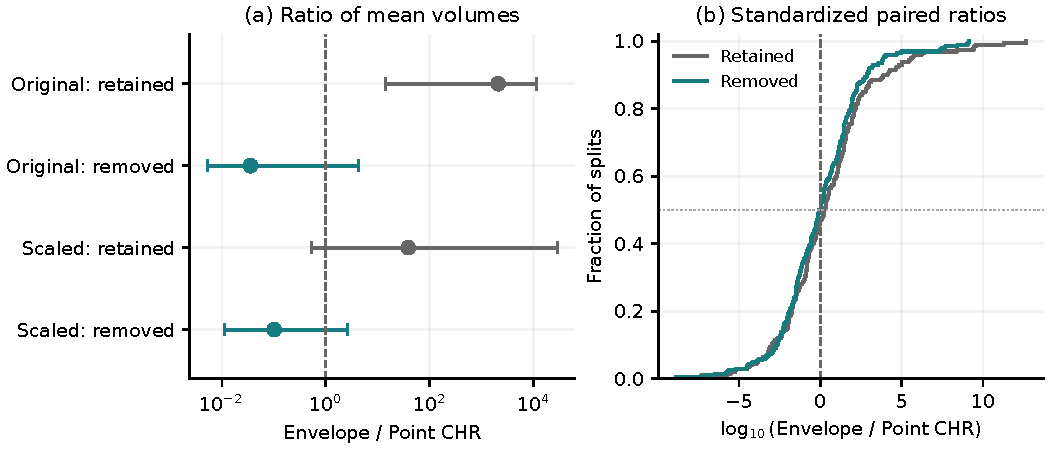
\includegraphics[width=\linewidth]{crime_comparison.pdf}
\caption{Crime mean and paired-ratio diagnostics. Panel (a) shows $R$ with
20,000 paired split-bootstrap percentile intervals on a logarithmic axis.
Panel (b) shows empirical cumulative distributions of standardized split-level
log ratios. Ratios below one (log ratios below zero) favor envelope. The apparent
mean advantage after deletion is much larger than the typical-split advantage.}
\label{fig:crime}
\end{figure}

\section{Mechanism, influential tails, and coverage}\label{sec:mechanism}
For calibration residual coordinate $j$, envelope uses statistics of the form
\begin{equation}
 m_j=\frac{1}{n}\sum_{i=1}^{n}e_{ij},\qquad
 s_j^2=\frac{1}{n}\sum_{i=1}^{n}(e_{ij}-m_j)^2,
 \label{eq:calibration}
\end{equation}
within its candidate-augmented surface construction \cite{methodnote}.
An extreme residual can affect both statistics even when the forest's targets
were standardized during training. Because Equation~\eqref{eq:volume}
multiplies widths across coordinates, moderate coordinate inflation can become
a large volume effect in 18 dimensions. This explains a plausible mechanism;
it is not a claim that every extreme residual necessarily increases every width.

\begin{table}[htbp]
\centering\small
\caption{Envelope mean volume by the original partition of the removed row.
Both datasets use standardized target training. Test-only deletion leaves
training and calibration unchanged, providing an exact control.}
\label{tab:partitions}
\begin{tabular}{llrrr}
\toprule
Dataset & Original partition & Splits & Retained mean volume & Removed mean volume\\
\midrule
rf2 & Training & 158 & 81,887.1 & 14,890.8 \\
rf2 & Calibration & 6 & 1,143,702.3 & 8,621.9 \\
rf2 & Testing & 36 & 14,828.6 & 14,828.6 \\
Crime & Training & 143 & $4.902\times 10^{62}$ & $3.336\times 10^{62}$ \\
Crime & Calibration & 11 & $1.285\times 10^{67}$ & $1.092\times 10^{60}$ \\
Crime & Testing & 46 & $1.513\times 10^{63}$ & $1.513\times 10^{63}$ \\
\bottomrule
\end{tabular}
\end{table}

For Crime, only 11/200 splits place the largest community in calibration,
but these account for 99.90\% of the retained standardized envelope's total
volume. Their mean volume drops from $1.285\times10^{67}$ to
$1.092\times10^{60}$ on deletion. The five largest retained-envelope trials
contribute 99.28\% of total volume. In contrast, the median paired envelope
volume reduction from deletion is only 0.274\%. Figure~\ref{fig:tail} makes
this difference between average and typical behavior visible.

\begin{figure}[htbp]
\centering
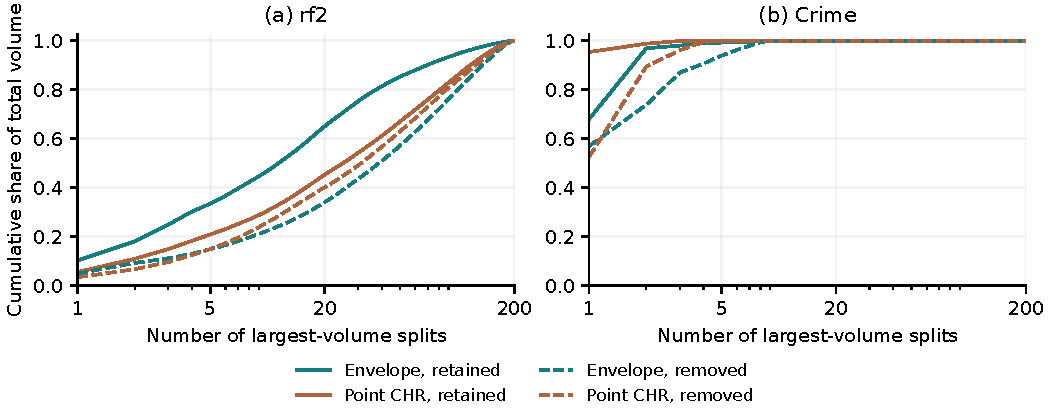
\includegraphics[width=\linewidth]{tail_concentration.pdf}
\caption{Concentration of volume across the 200 splits, with standardized
training. Each curve sorts its own split volumes from largest to smallest
and plots their cumulative share of the total. Rapid saturation means that
few splits dominate the arithmetic mean. The horizontal axis is logarithmic;
the split ordering can differ between methods and conditions.}
\label{fig:tail}
\end{figure}

\begin{table}[htbp]
\centering\small
\caption{Paired deletion effects with standardized training. Reductions are
percentages; coverage changes and their Monte Carlo intervals are percentage
points on the identical remaining test observations. Positive reductions
indicate smaller regions after deletion.}
\label{tab:effects}
\begin{tabular}{llrrrr}
\toprule
& & \multicolumn{2}{c}{Volume reduction (\%)} & \multicolumn{2}{c}{Common-test coverage}\\
\cmidrule(lr){3-4}\cmidrule(lr){5-6}
Dataset & Method & Mean & Paired median & Change & 95\% interval\\
\midrule
rf2 & Envelope & 85.550 & 46.444 & +0.0059 & [-0.130, +0.142] \\
rf2 & Point CHR & 37.923 & 17.165 & -0.0846 & [-0.286, +0.116] \\
Crime & Envelope & 99.917 & 0.274 & -0.0630 & [-0.252, +0.126] \\
Crime & Point CHR & 68.337 & 0.000 & +0.0367 & [-0.216, +0.290] \\
\bottomrule
\end{tabular}
\end{table}

\section{Outlier status and relevance of other cohorts}
The rf2 observation is exceptionally isolated relative to the rest of its
target distribution. Crime's largest community is better described as an
influential upper-tail observation. Its maximum robust z-score across
$\log(1+y)$-transformed targets is 6.696, followed by 6.405 and 6.120 for
the next two observations under the same statistic. These transformed scores
are descriptive and should not be compared numerically with rf2's raw-target
z-score as a universal severity scale.

In Crime, the community has the largest value for seven of the eight count
outcomes, but its population-based rates are less exceptional. For example,
its larceny count is 235,132, the cohort maximum, whereas its larceny rate
is at approximately the 54th empirical percentile. Its nonviolent-crime rate
is at approximately the 74th percentile. This is consistent with a city-size
effect rather than an isolated spike across all outcomes. It does not verify
the record's accuracy. Removing a legitimate large community changes the
benchmark population, so the analysis is labeled a largest-community sensitivity
experiment rather than a corrected-data experiment.

\begin{table}[htbp]
\centering\small
\caption{Screen of the eight existing cohorts under the complete-data,
original-training benchmark at nominal 90\% coverage. $N$ is the retained
cohort size and $d$ the number of outputs. These ratios precede the new
standardized controls; they must not be mixed with the standardized result tables.}
\label{tab:screen}
\begin{tabular}{lrrrp{6.4cm}}
\toprule
Dataset & $N$ & $d$ & Env./CHR mean volume & Assessment\\
\midrule
stock & 315 & 6 & Unbounded CHR & CHR is unbounded with the small calibration sample. \\
rf2 & 7,679 & 8 & 6.954 & Isolated extreme value; no standardized reversal. \\
scm1d & 9,803 & 16 & 0.535 & Envelope already has smaller mean volume. \\
scm20d & 8,966 & 16 & 0.508 & Envelope already has smaller mean volume. \\
energy & 768 & 2 & 0.776 & Envelope already smaller; building simulations \cite{energy}. \\
student & 649 & 3 & 0.282 & Envelope already smaller; student records \cite{student}. \\
air & 6,941 & 4 & 0.983 & Envelope slightly smaller; hourly series \cite{air}. \\
crime & 1,902 & 18 & 2,081.972 & Community records; fixed deletion tested \cite{crime}. \\
\bottomrule
\end{tabular}
\end{table}

Only rf2 and Crime start with larger envelope mean volume in this screen.
The remaining finite-baseline cohorts already favor envelope on that metric.
Energy is generated from building simulations; Student contains student-level
records; Air is an hourly time series. Stock has an unbounded corrected CHR
region in all 200 splits because its calibration halves are too small for
the required finite conformal quantile. These facts limit their suitability
for the requested finite-baseline loss-to-win example. The screen is
descriptive: deletion fits were run for rf2 and Crime, not for all eight
cohorts or every possible removal rule.

\subsection{Interpretation for reporting the experiments}
The strongest supported rf2 statement is that a single statistically extreme
observation substantially inflates envelope's mean volume even with
training-target standardization, while its removal leaves coverage almost
unchanged and does not reverse the CHR comparison. Crime provides the requested
reversal in empirical mean volume, but the gain is concentrated in rare
calibration-tail cases and is not established as a consistent advantage across
splits. These outcomes support a focused claim about sensitivity to influential
observations. They do not support a general rule that outlier removal makes
envelope outperform Point CHR, or that deletion is warranted in the primary
benchmark.

\appendix
\section{Calibration details, uncertainty, and reproducibility}
\subsection{Point CHR and the corrected order statistic}
For a calibration multiset $v=(v_1,\ldots,v_m)$, define
\begin{equation}
 \Q(v)=
 \begin{cases}
 v_{(r)}, & r=\lceil(m+1)(1-\alpha)\rceil\le m,\\
 +\infty, & r>m.
 \end{cases}
\end{equation}
Point CHR randomly divides the calibration residuals into two halves,
$A$ and $B$, using seed 42. With $q_j=\Q(\{e_{ij}:i\in A\})$, its thresholds are
\begin{equation}
 u_j^{\CHR}=q_j\,
 \Q\!\left(\left\{\max_k\frac{e_{ik}}{q_k}:i\in B\right\}\right).
\end{equation}
Each quantile uses its own sample size. The original 95-row Crime calibration
set gives halves of 47 and 48 observations; deleting a calibration row gives
47 and 47. The original rf2 calibration halves are 192 and 192; calibration-row
deletion gives 191 and 192. The same seeded splitting procedure is rerun on
the reduced calibration array, so internal CHR half membership need not remain
identical after deletion. This is part of applying the fixed procedure to
the reduced data; outer train/calibration/test memberships remain matched.

The current analysis consistently uses the corrected second-half recalibration
rank. Historical raw Crime archives preserve pre-correction CHR bounds; their
residual arrays, rather than their obsolete CHR bounds, are reused for this
comparison. No alternative rank was selected to improve envelope's ranking.

\subsection{Monte Carlo summaries and their limits}
Coverage bars and paired coverage-change intervals use split-level standard
deviations and the normal approximation $1.96\,\mathrm{SD}/\sqrt{200}$.
Crime mean-volume intervals use 20,000 bootstrap samples of the 200 split
indices with replacement, random seed 20260909, retaining method and treatment
pairing. The 2.5th and 97.5th percentiles of the bootstrap ratios form the
reported intervals. All such uncertainty summaries are conditional on the
fixed dataset and random-split protocol. They do not represent uncertainty
from drawing a new population sample, account for cohort selection, or resolve
the effects of rare extreme splits not observed among the 200 trials.

rf2's row was identified after examining its outcomes, and Crime was investigated
after screening existing method results. These are exploratory sensitivity
analyses, not preregistered confirmatory tests. The Crime deletion rule was fixed
before its deletion results were computed. The nominal 90\% level is a target;
near-nominal empirical coverage under these splits does not by itself establish
exchangeability or validate forecasting claims.

\subsection{Completed work and audit trail}
The rf2 audit verifies original source hashes, exact deletion alignment,
training-only centers and scales, retained method metrics, and independently
recomputed removed-condition metrics. All 36 test-only deletion pairs reproduce
their bounds. Crime contains 800 fitted conditions (600 new and 200 reused).
Its fit audit checks deletion membership and training transformations; its
reporting audit recomputes calibration bounds and all 1,600 method coverage and
volume records. Across 46 test-only deletion splits, two training choices,
and two methods, all 184 bound comparisons reproduce exactly. Source and
archive checksums are retained. Source observations and primary benchmark
results were not overwritten. No additional model fitting was performed to
prepare this report.

The portable report folder contains the complete \texttt{.tex} source,
vector PDF figures, the compiled report, selected CSV/JSON evidence under
\texttt{data/}, and a manifest of source checksums. Full fitted residual archives
remain in the project. The source locations relative to the project root are:
\begin{itemize}
\item \path{envelope_method/results/rf2_standardized_outlier_control/}
\item \path{envelope_method/results/rf2_remaining/model_time/}
\item \path{envelope_method/results/real_outlier_screen/crime_control/}
\item \path{envelope_method/results/real_comparison_audited.csv}
\end{itemize}
The report builder is \path{envelope_method/build_outlier_sensitivity_report.py}.
It verifies summary statistics against trial data and regenerates tables and
figures. The report source can be compiled from its folder with
\texttt{pdflatex} twice, or with \texttt{tectonic}.

\clearpage
\begin{thebibliography}{9}\small\raggedright
\setlength{\itemsep}{2pt}\setlength{\parskip}{0pt}
\bibitem{methodnote} Project method note.
\emph{Signed Surface-Envelope Transductively Standardized Conformal Prediction:
Construction, finite-sample proofs, and comparison with the separated shortcut}.
September 8, 2026. Source: \path{envelope_method/signed_envelope.tex}.
\bibitem{mulan} Mulan project. \emph{Multi-target regression datasets},
including River Flow 2.
\url{https://mulan.sourceforge.net/datasets-mtr.html}.
\bibitem{crime} UCI Machine Learning Repository.
\emph{Communities and Crime Unnormalized}, dataset 211.
\url{https://archive.ics.uci.edu/dataset/211/communities+and+crime+unnormalized}.
\bibitem{energy} UCI Machine Learning Repository.
\emph{Energy Efficiency}, dataset 242.
\url{https://archive.ics.uci.edu/dataset/242/energy+efficiency}.
\bibitem{student} UCI Machine Learning Repository.
\emph{Student Performance}, dataset 320.
\url{https://archive.ics.uci.edu/dataset/320/student+performance}.
\bibitem{air} UCI Machine Learning Repository.
\emph{Air Quality}, dataset 360.
\url{https://archive.ics.uci.edu/dataset/360/air+quality}.
\end{thebibliography}
\end{document}
